\documentclass[11pt,a4paper]{article}

\usepackage[T1]{fontenc}
\usepackage[utf8]{inputenc}
\usepackage[frenchb]{babel} % Global stuff set to french
\usepackage[margin=2.5cm]{geometry} % The margin of the page
% \usepackage{amsmath}  % to include math formulas
\usepackage{graphicx} % to include pictures
\usepackage[hidelinks]{hyperref} % To include hyperlinks in a PDF
\usepackage{fancyhdr} % to be able to make the page fancy looking
\usepackage{appendix} % To make appendixes
\usepackage{color} % For text colors
\usepackage{palatino} % Change font
% \usepackage{tabularx}
\usepackage{subcaption}
\usepackage{enumitem}
\usepackage{changepage}
\usepackage[nonumberlist, nopostdot, numberedsection, toc]{glossaries}
\usepackage{imakeidx}
\makeindex
\makenoidxglossaries

%% Fancy layout
\pagestyle{fancy}
\lhead{Projet d'année - Wizard Poker}
\chead{}
\rhead{Groupe 2}
\lfoot{}
\cfoot{}
\rfoot{Page \thepage}
\renewcommand{\headrulewidth}{0.4pt}
\renewcommand{\footrulewidth}{0.4pt}

%%% Glossary

\newglossaryentry{deck}{
  name=Deck,
  description=Un deck est un ensemble de 20 cartes
}

\newglossaryentry{collection}{
  name=Collection,
  description=Ensemble qui contient toutes les cartes disponibles et
  connues par le jeu
}

\newglossaryentry{tchat}{
  name=Tchat,
  description=Messagerie instantanée permettant à 2 personnes de
  s'échanger des messages écrit
}

\newglossaryentry{visiteur} {
  name=Visiteur,
  description=Personne n'ayant pas encore de compte
}

\newglossaryentry{label1}{name=example1, description=description1}
\newglossaryentry{label2}{name=example2, description=description2}


%%% --- %%% --- DOCUMENT START --- %%% --- %%%
\begin{document}
\begin{titlepage}

\topskip0pt
\begin{center}
    \vspace*{\fill}
        \hrule
        \vspace*{2pt}
        \hrule
        \vspace*{15pt}
        \textsc{\Huge{INFO-F106 : Projet d'année \\\vspace*{8pt} Rappport intermédiaire}}
        \vspace*{15pt}
        \hrule
        \vspace*{2pt}
        \hrule
  \vspace*{\fill}
\end{center}
\null
\vfill
  
\large{Mardi 16 décembre 2014} \hfill \large{Carlos Requena López - \emph{410031}}

\end{titlepage}
\pagestyle{empty}
\tableofcontents
\newpage
%%% Counting pages now %%%
\pagestyle{fancy}

\setcounter{page}{1}

\section{Introduction}
\label{sec:intro}

\subsection{But du projet}
\label{sec:but}

Dans le cadre du projet d'analyse et méthode et de système
d'exploitation, il est demandé d'implémenter un jeu de carte en ligne
de type HeartStone.

\medbreak

Ce projet devra fournir un jeu de carte symétrique où deux joueurs
pourront s'affronter et gagner des points pour un classement
général. Chaque joueur disposera d'un ensemble de cartes avec lequelles
il pourra affronter ses adversaires. Ces cartes pourront être des
créature qui peuvent attaquer et des cartes de type
sort qui lanceront des événements spéciaux.

\medbreak

Le projet fournira à l'utilisateur une interface intuitive, un gestionnaire
d'amis, un service de tcaht pour pouvoir rester en contact avec eux ainsi
qu'un classement générale où chaque joueurs pourra comparer ses résultas avec
les autres.

\medbreak

Le Wizard Poker sera disponible à n'importe quel joueurs enregistré
pour jouer contre d'autres joueurs et essayer de gagner des places
dans le classement générale. Il permettra aussi à de nouveaux joueurs
de consulter ce classement et de s'enregistrer en tant que nouveau
joueur. Dans ce cas, le joueur recevra ses premières cartes et sera
invité à confectionner son premier deck avant d'affronter son premier
adversaire.

\subsection{Historique du document}
\label{sec:hist}


\begin{table}[h]
  \centering
  \begin{tabular}[ht]{|l|l|l|p{18em}|}
    \hline

    \textbf{Version}
    & \textbf{Auteur}
    & \textbf{Date modification}
    & \textbf{Description des changements}\\ \hline \hline
    NEXT &  &  &  \\ \hline
    NEXT &  &  &  \\ \hline
     v0.6 & Corentin Candeur & 16/12/15 & Deuxième relecture, corrections orthographiques/syntaxiques et diverses petites corrections \\ \hline
    v0.5 & Rémy Detobel & 14/12/15 & Première relecture, diverses petites corrections \\ \hline
    v0.4 & Carlos Requena  & 13/12/15 22h00 & Ajout d'un système de glossaire \\ \hline
    v0.3 & Rémy et Lucie  & 11/12/15 16h20 & Ajout de diagrammes, ajout de ``Exigences du domaine'' \\ \hline
    v0.2 & Amin et Maxime & 10/12/15 23:45 & Ajout de la partie ``Exigences fonctionnelles''\\ \hline
    v0.1 & Jonas et Raphaël & 10/12/15 13:28 & Ajout de la partie ``But du projet''\\ \hline
    v0.0 & Carlos Requena & 26/11/15 22:30 & Mise en place du document.Ajout des diagrammes réalisés en groupe le 25/11/15.\\ \hline
  \end{tabular}
  \caption{Changements document}
  \label{tab:hist}
\end{table}


\glsaddall
\printnoidxglossaries


\section{Besoins de l'utilisateur}
\label{sec:besoins}

Le Use Case Diagram montre les différentes interactions entre les
utilisateurs et le programme.  Nous pouvons voir ici deux utilisateurs
différents.  Le visiteur est un utilisateur n'ayant pas de compte et ses
actions sont donc très limitées et consistent seulement en la création d'un compte.
Nous avons aussi le joueur qui est l'utilisateur principal du Wizard Poker.
C'est lui qui va interagir avec le jeu.

\subsection{Exigences fonctionnelles}
\label{sec:exi-fonc}
\begin{figure}[ht]
  \centering
  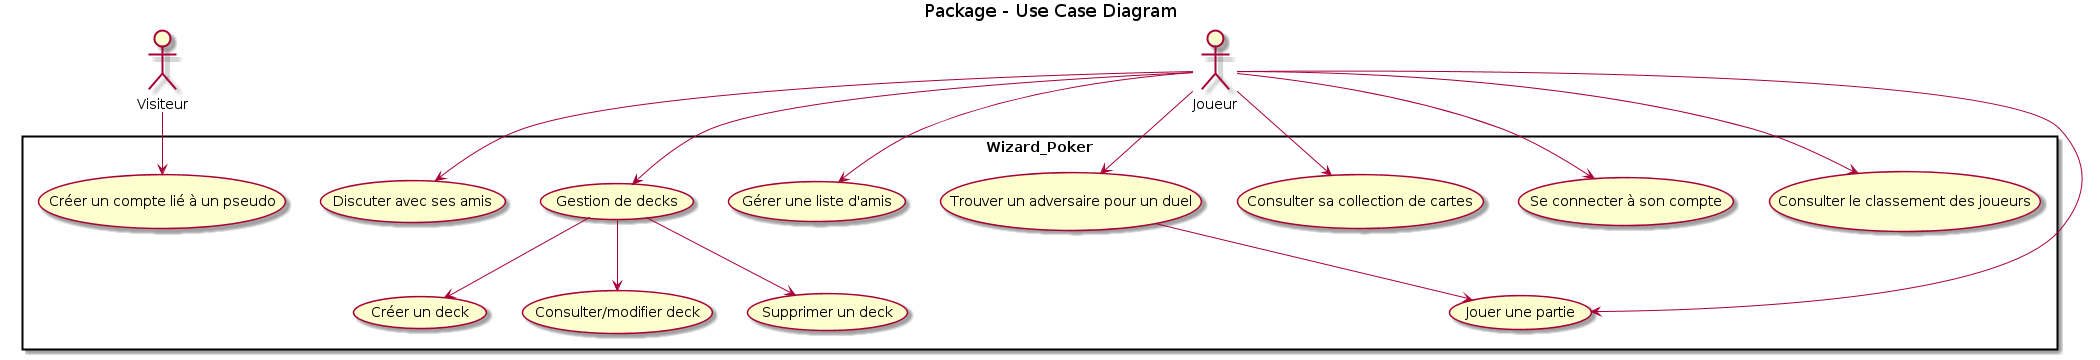
\includegraphics[width=1\textwidth]{../uml_files/UseCaseDiagram.png}
  \caption{\label{fig:usecasebesoin} Use Case Diagram}
\end{figure}

\subsubsection*{Créer un compte lié à un pseudo}

Tout visiteur se aura la possibilité de se créer un compte
lié à un pseudo (si ce dernier est disponible) afin de pouvoir
profiter pleinement du jeu.


\subsubsection*{Se connecter à son compte}

Le joueur devra se connecter à son compte s'il souhaite effectuer
les différentes actions répertoriées ci-dessous.


\subsubsection*{Consulter sa collection de cartes}

Le joueur peut consulter l'ensemble des cartes présentes dans sa
collection. Pour cela, il devra au préalable s'être connecté.


\subsubsection*{Gestion de decks}

Un deck est un ensemble de cartes qui sera utilisé par le joueur
lors d'un duel. Plusieurs actions peuvent être effectuées sur les
decks telles qu'en supprimer un ou plusieurs, les consulter, les
modifier ou tout simplement en créer un nouveau.


\subsubsection*{Gérer une liste d'amis}

Chaque joueur aura une liste d'amis avec lesquels il pourra
interagir s'il le souhaite. Il pourra aussi ajouter ou supprimer un ami de sa liste.


\subsubsection*{Discuter avec ses amis}

Le joueur pourra, à tout moment, parler avec un ou plusieurs de ses
amis actuellement connectés. Pour cela, un tchat sera mis à
disposition du joueur.  Le joueur pourra donc communiquer avec ses
amis par message à tout moment. Cependant un joueur ne peut communiquer qu'avec une personne à la fois.
\subsubsection*{Proposer une partie à un ami}

Si le joueur le souhaite, il peut proposer une partie à un de ses
amis connectés. Ce dernier est libre d'accepter ou non cette demande.
S'il l'accepte la partie est lancée entre les deux joueurs.


\subsubsection*{Trouver un adversaire pour un duel}

Lorsqu'un joueur voudra lancer une partie, le jeu trouvera
automatiquement un adversaire dans la liste des personnes
connectées. Le choix de l'adversaire est totalement aléatoire.


\subsubsection*{Consulter le classement}

Le classement va permettre de classer les joueurs en fonction de
leur nombre de victoires et de défaites. Ce classement se
basera donc sur le ratio victoires/défaites.


\subsection{Exigences non fonctionnelles}
\label{sec:exi-nonfonc}

Dans le cadre de ce projet nous allons d'abord implémenter les exigences fonctionnelles.  Nous verrons ensuite pour ajouter les exigences non fonctionnelles.


\subsubsection*{Ergonomie}
Créer un jeu qui sera simple d'utilisation et facilement compréhensible pour un utilisateur n'ayant jamais joué à un jeu de ce genre.\\
Pour cela, on peut rendre l'interface intuitive à l'aide de ``boutons'' décrivant exactement leur utilité ou encore à l'aide d'un rapide tutoriel après la création du compte expliquant les différentes caractéristiques du jeu.


\subsubsection*{Design}
Le design est l'apparence qu'aura l'interface graphique. Comme pour le point précédent, une belle interface va permettre à l'utilisateur de facilement voir les différentes possibilités offertes par le jeu en plus d'apprécier l'esthétique.\\
Le design est un ``domaine'' (vague) c'est-à-dire qu'il définit l'apparence du jeu mais aussi les différents sons et/ou musiques.


\subsubsection*{S'amuser}
Qu'est-ce qu'un bon jeu?\\
Un bon jeu est un jeu attractif, beau, facile à comprendre mais avant tout, un bon jeu est un jeu où l'on s'amuse. Notre principal objectif sera de réaliser ce jeu et de permettre à tous les joueurs de s'amuser.


\subsection{Exigences de domaine}
\label{sec:exi-dom}

Le domaine du jeu vidéo laisse beaucoup de liberté.  En effet, chaque créateur essaye de créer son univers, de développer son concept.  Cependant, tous les jeux doivent permettre à leur utilisateur de trouver du plaisir ou une certaine forme de satisfaction.  Il faut également éviter que le joueur soit interrompu durant sa partie.  Les exigences du domaine ne sont donc pas nombreuses mais compliquées à satisfaire complètement.

Le Wizard Poker est un jeu de cartes.  Ce type de jeu impose lui aussi quelques contraintes.  Il faut éviter que les cartes soient trop fortes.  Pour la durée de vie du jeu il faut aussi faire en sorte qu'il y ait un nombre conséquent de cartes.  N'oublions pas enfin le temps de jeu.  En effet, une partie de cartes dure rarement longtemps pour éviter l'ennui.

Pour résumer, un utilisateur attend de l'amusement, un jeu équilibré et une stabilité acceptable (voir infaillible coté serveur).  Nous nous concentrerons dans un premier temps (dans le cadre de ce projet) à ce troisième point et nous verrons pour satisfaire à 100\% les ``gamers`` dans un second temps.



\section{Besoins du système}
\label{sec:besoins-sys}

\subsection{Exigences fonctionnelles}
\label{sec:exi-fonc-sys}

% Ce type d’exigences sera décrit en utilisant des diagrammes use
% case et en fournissant une description *plus détaillée* pour
% chacun d’entre eux (comme vu au cours théorique et aux exercices).

Sequence diagram pour interaction??

Le système doit interagir avec l'utilisateur, et lui proposer
certaines actions, comme commencer un duel, gérer ses \index{deck}s,
consulter le classement des joueurs, etc.

Pour les nouveaux joueurs, l'application doit offrir la possibilité de
s'enregistrer, avec un pseudonyme et un mot de passe.


\subsection{Exigences non fonctionnelles}
\label{sec:exi-nonfonc-sys}

Les exigences non fonctionnelles décrivent le comportement de
l'application.

Le système doit être tout d'abord robuste et stable, c'est-à-dire
gérer les erreurs et éviter les crashs et les déconnexions... Il doit
par ailleurs être agréable d'utilisation pour l'utilisateur (ergonomie
et esthétique/design) et garantir que celui-ci ne puisse pas tricher
pendant une partie.

Donc en résumé, robuste, stable, sûr, et excessivement amusant. Des
heures de franche rigolade, en toute sécurité, sont assurées à tout
utilisateur du jeu.

\subsection{Design et fonctionnement du système}
\label{sec:design}

Afin de mieux présenter le fonctionnement du programme voici quelques diagrammes où vous pouvez voir la manière dont nous allons essayer de développer Wizard Poker.
% Cette partie sera décrite à l’aide des différents diagrammes UML
% vus au cours théorique et aux exercices.


% Peut être le supprimer vu qu'il est déjà  plus haut
\begin{figure}
  \centering
  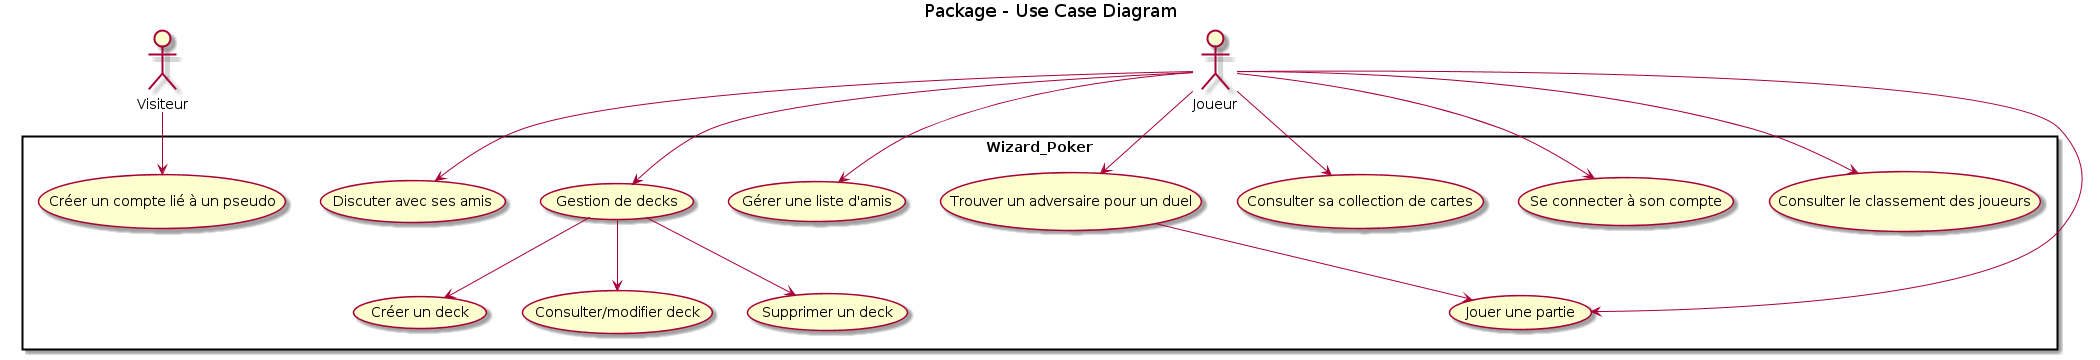
\includegraphics[width=1\textwidth]{../uml_files/UseCaseDiagram.png}
  \caption{\label{fig:usecase} Use Case Diagram du jeu en question}
\end{figure}

\begin{figure}[ht]
  \centering
  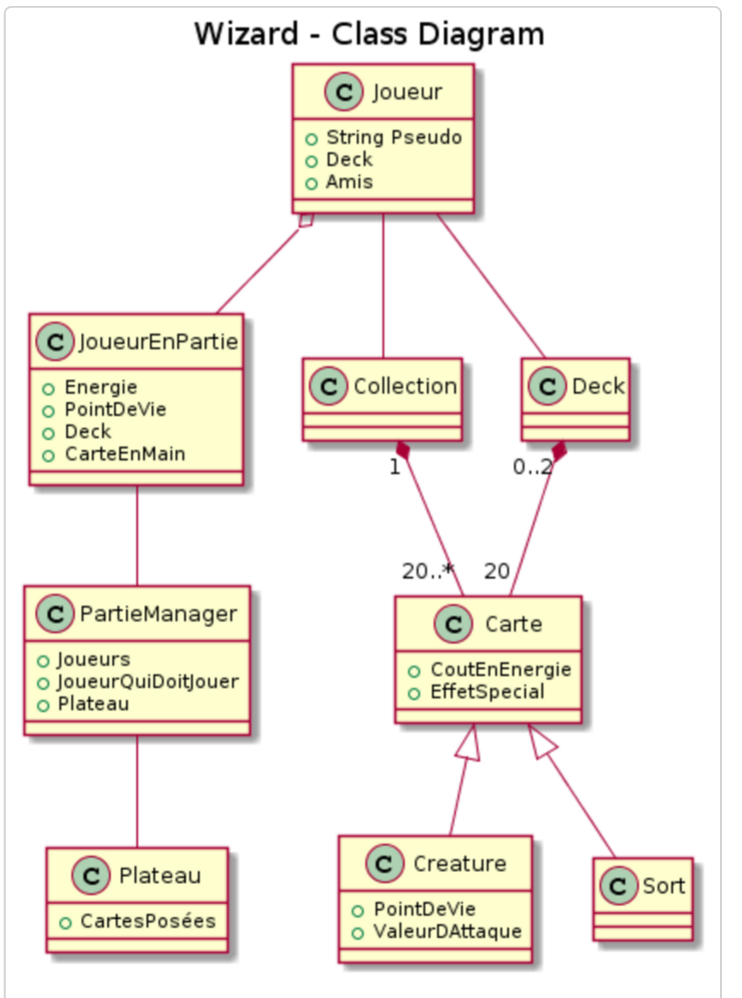
\includegraphics[width=1\textwidth]{../uml_files/ClassDiagram.png}
  \caption{\label{fig:class} Diagramme des classes}
\end{figure}

\subsubsection{Diagramme de séquence}
Ce diagramme de séquence vise à montrer la manière dont un joueur va pouvoir initialiser une partie.  Les diagrammes d'activités vont permettre de détailler la manière dont une partie se déroule.
\begin{figure}[ht]
  \centering
  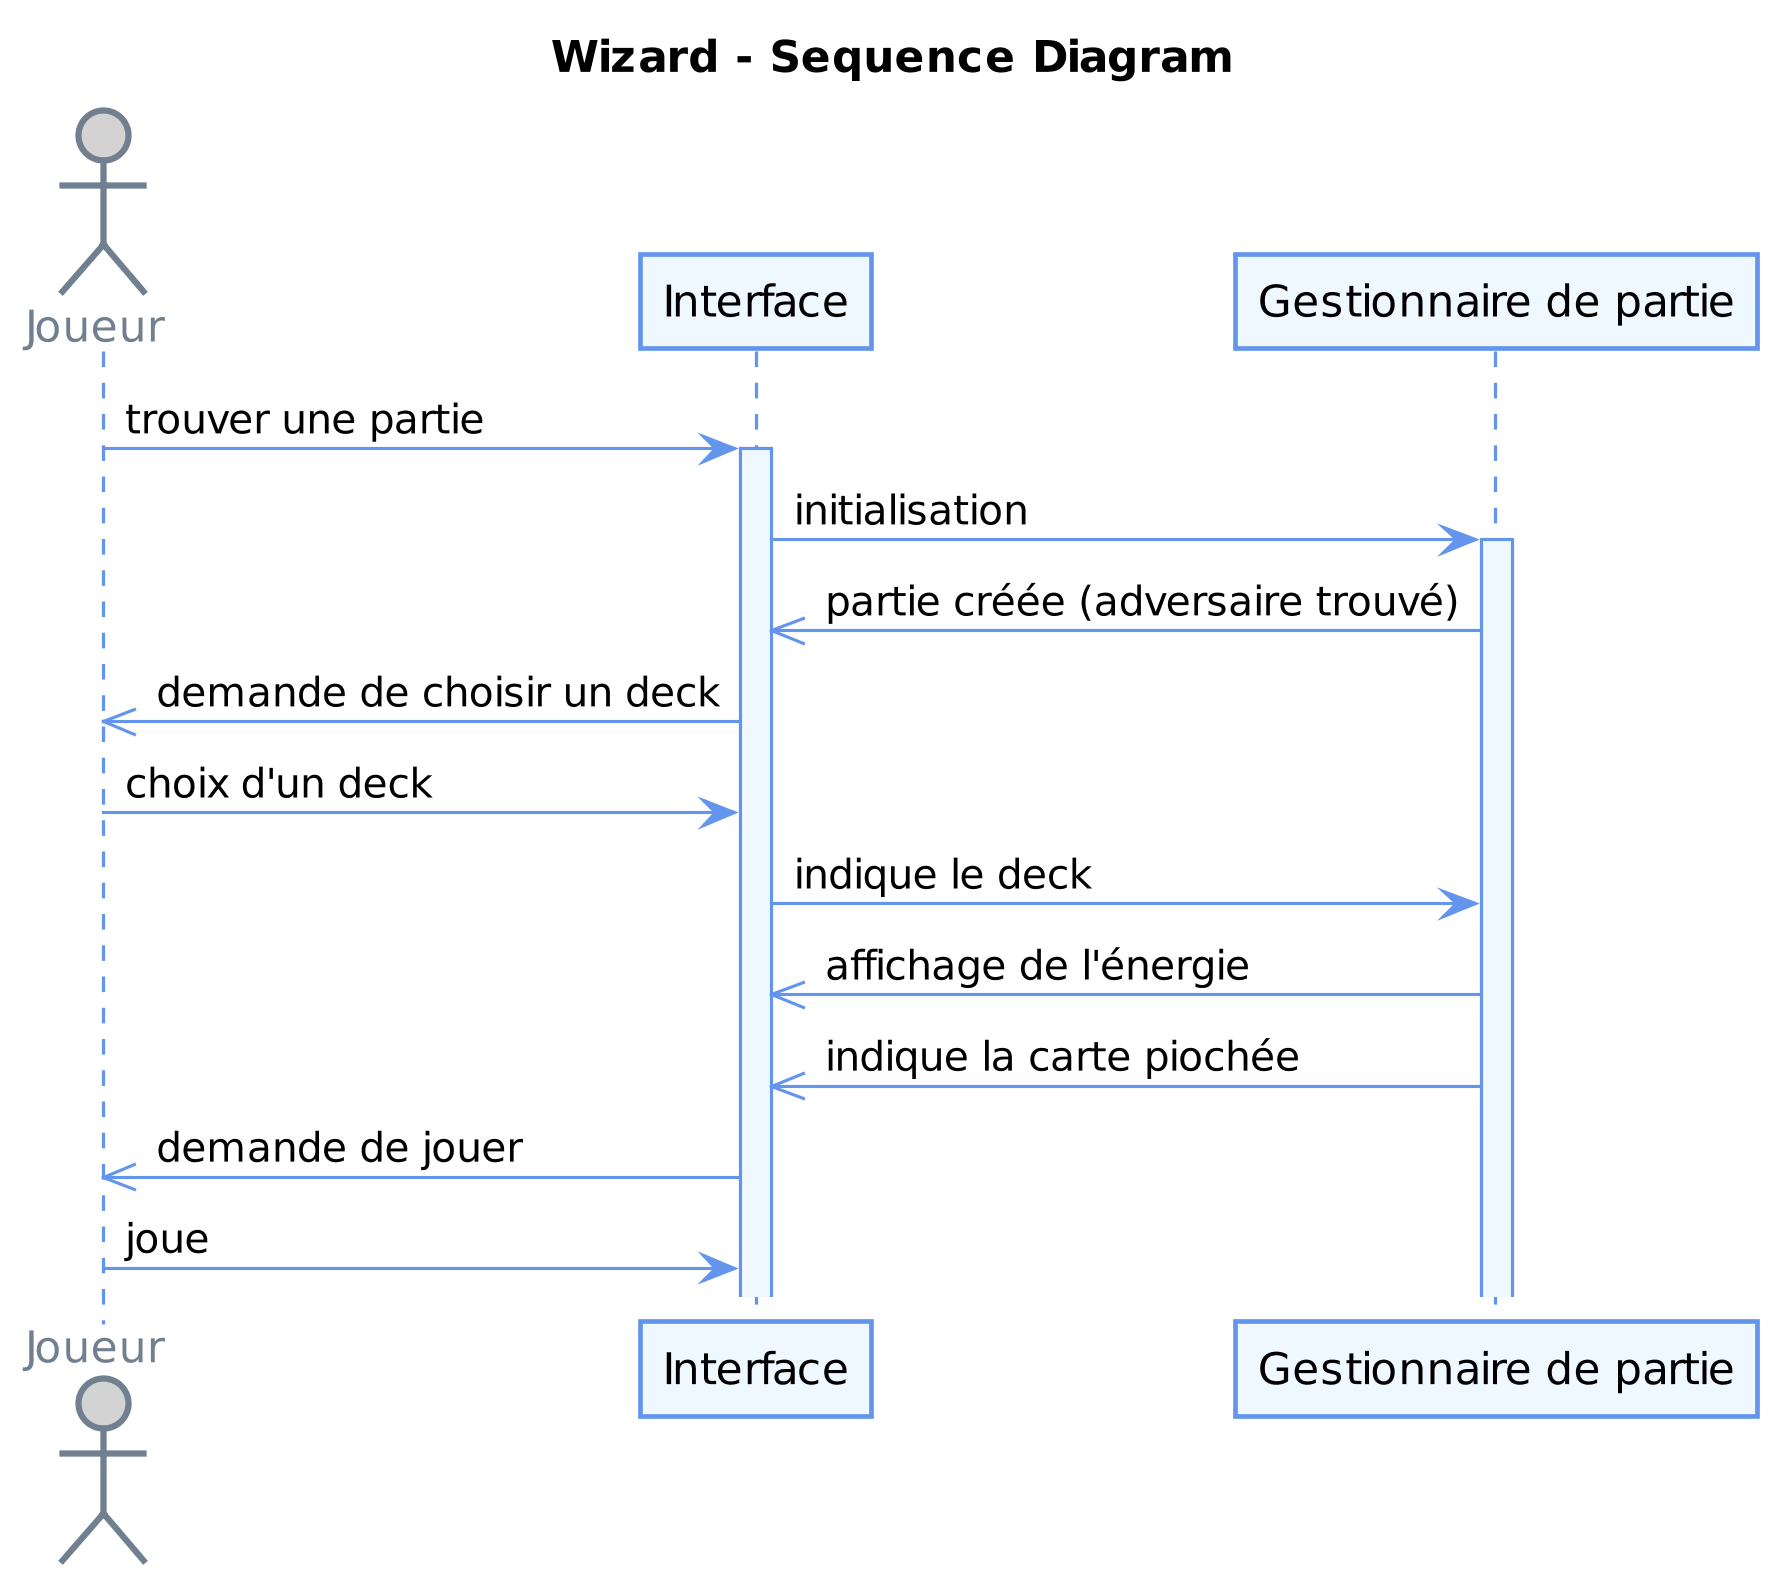
\includegraphics[width=1\textwidth]{../uml_files/SequenceDiagram.png}
  \caption{\label{fig:seq} Diagramme de séquence}
\end{figure}

\subsubsection{Diagramme d'activité}
Le but de ces deux diagrammes d'activité est de décrire comment va se dérouler une partie.
\begin{figure}[ht]
  \centering
  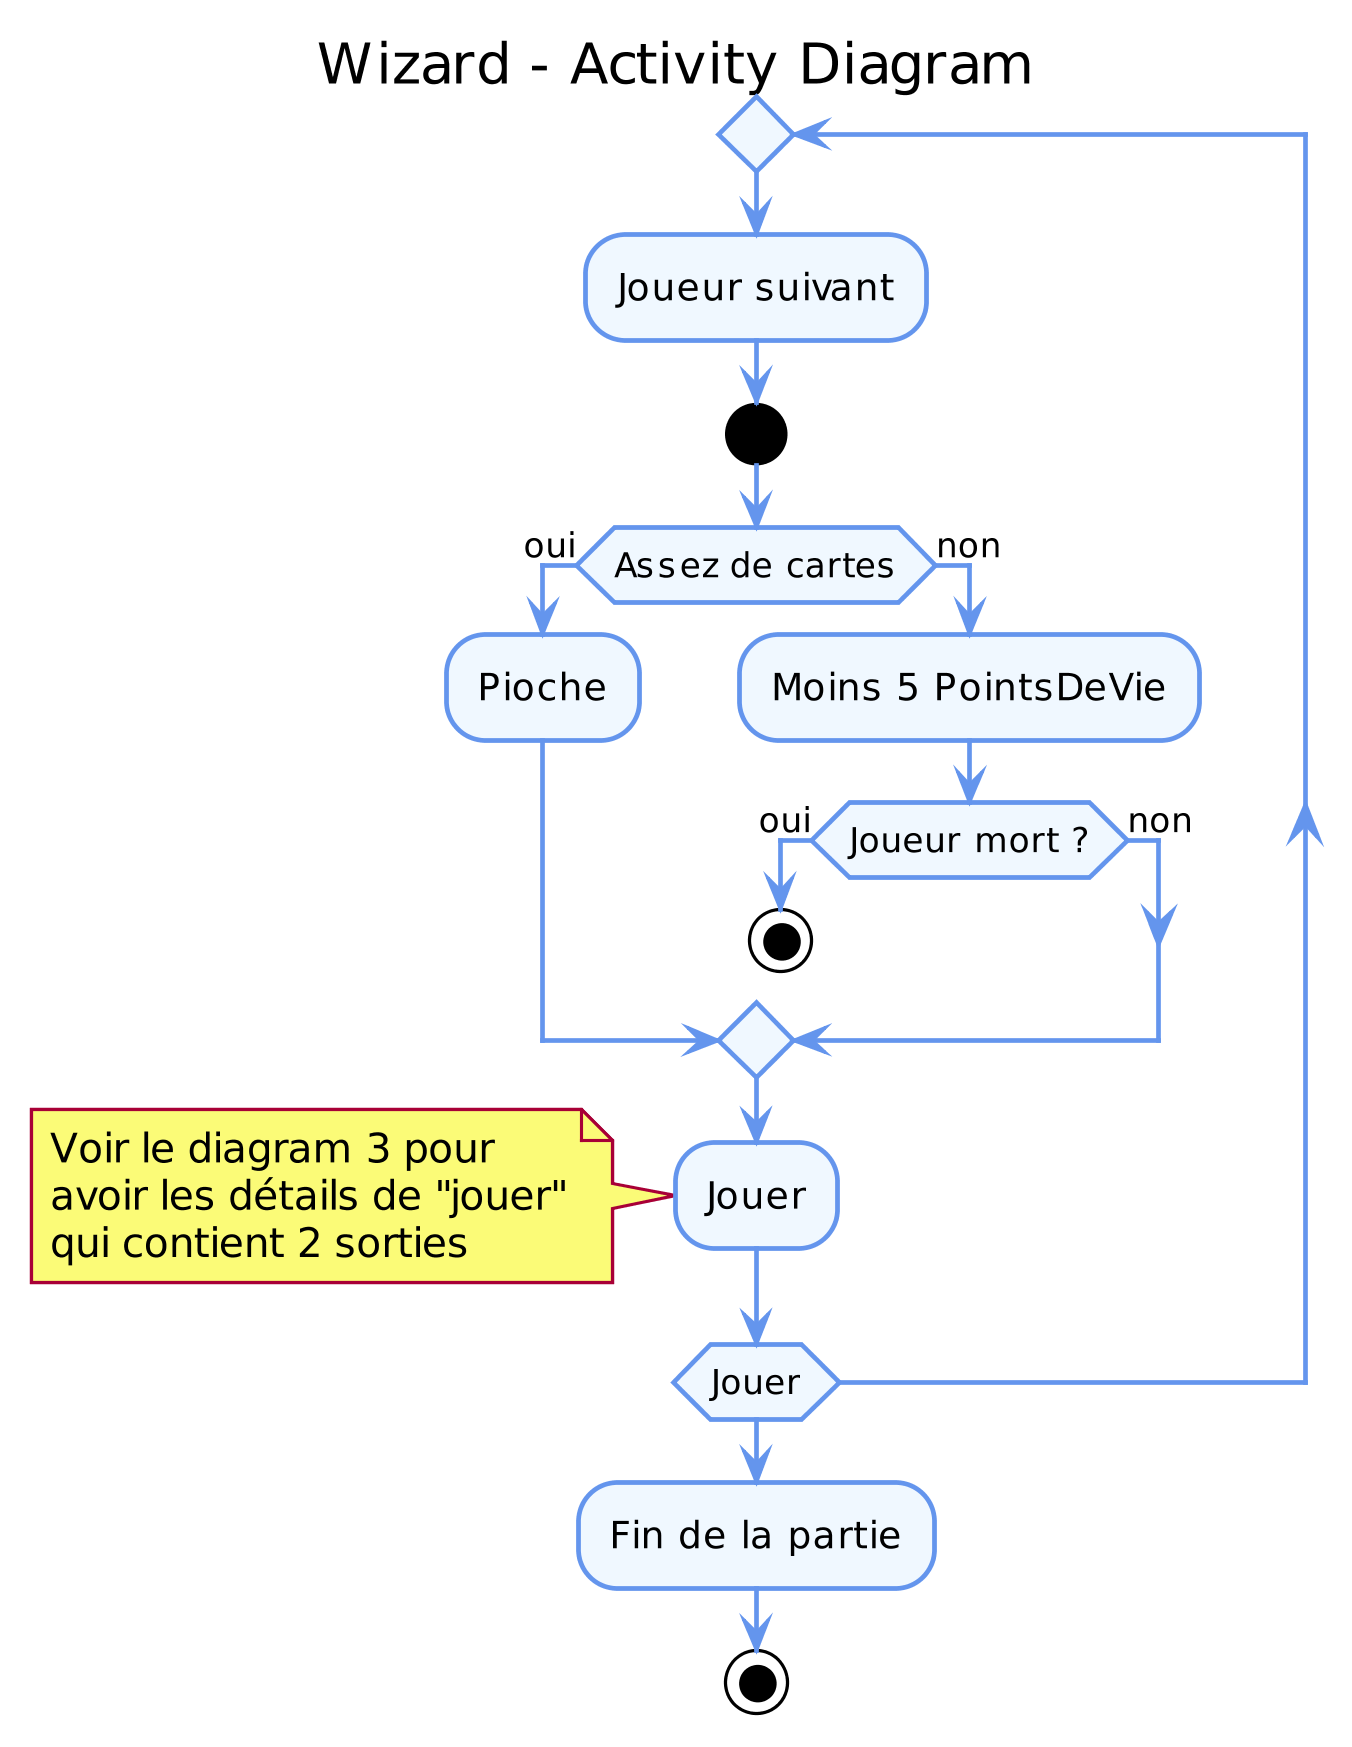
\includegraphics[width=1\textwidth]{../uml_files/ActivityDiagram.png}
  \caption{\label{fig:act1} Diagramme d'activité}
\end{figure}

\begin{figure}[ht]
  \centering
  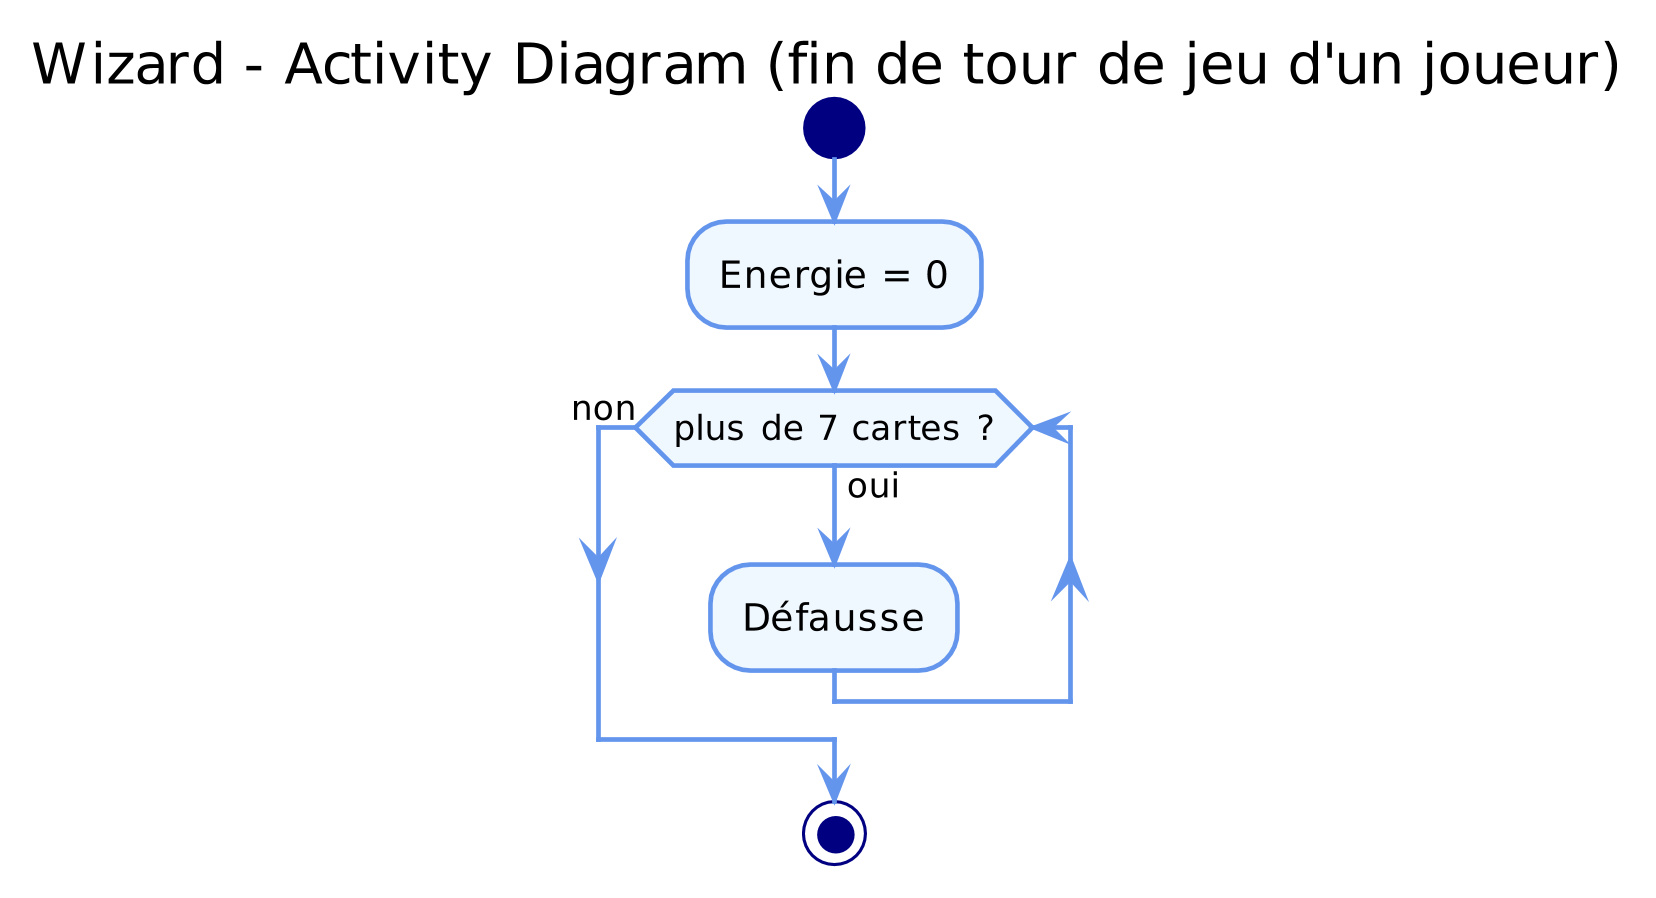
\includegraphics[width=1\textwidth]{../uml_files/ActivityDiagram2.png}
  \caption{\label{fig:act2} Diagramme d'activité 2}
\end{figure}

\clearpage
\printindex

\end{document}
